\documentclass[oneside]{book}

\usepackage{amsmath}
\usepackage{amssymb}
\usepackage{amsthm}
\usepackage{runic}
\usepackage{mathtools}
\usepackage{graphicx}
\usepackage{geometry}
\usepackage{makecell}
\usepackage{bigints}
\usepackage[breaklinks=true,pagebackref=true]{hyperref}

\usepackage{tkz-euclide}
%\usetkzobj{all}


\usepackage{tikz}
\usetikzlibrary{tikzmark}


\newcommand\tab[1][1cm]{\hspace*{#1}}
\newcommand\nextline{\newline\tab}
\newcommand\nextquestion{\newline\newline}
\newcommand\soln{$\text{sol}^\text{n}\text{ }$}
\newcommand\fs{\mbox{\large $\mathrlap{f}s\,$}\,}
\newcommand\thm[2]{\section{#1}\label{sec:#2}}
\newcommand\propn[2]{\section*{Proposition: #1}\label{sec:#2}\addcontentsline{toc}{section}{Proposition: #1}}
\newcommand\defn{\textbf{Definition}: }
\renewcommand\d[1]{\text{ d}#1}
\newcommand\ddx[1]{\frac{\text{d}}{\text{dx}}\left[#1\right]}
\newcommand\dfdx[2]{\frac{\text{d#1}}{\text{d#2}}}
\newcommand\dydx{\frac{\text{dy}}{\text{dx}}}
\newcommand{\Lim}[1]{\raisebox{0.5ex}{\scalebox{0.8}{$\displaystyle \lim_{#1}\;$}}}

\renewcommand\mod[1]{\text{ }\left(\text{mod }#1\right)}

\newcommand{\abs}[1]{\left\lvert#1\right\rvert}

\makeatletter
\Hy@AtBeginDocument{%
  \def\@pdfborder{0 0 1}% Overrides border definition set with colorlinks=true
  \def\@pdfborderstyle{/S/U/W 0.75}% Overrides border style set with colorlinks=true
                                % Hyperlink border style will be underline of width 1pt
}
\makeatother
\hypersetup{
    colorlinks=true,
    linkcolor=blue,
    linkbordercolor=blue,
    pdfborderstyle={/S/U/W 1}
}



\title{Introduction to Integration}
\author{Liam Gardner}
\date{\today}
\begin{document}
%\DeclarePairedDelimiter\abs{\lvert}{\rvert}

\renewcommand\cellgape{\Gape[4pt]}

\maketitle
\tableofcontents
\chapter{Introduction}
\section{Beginning Integration}
\tab
Integration is a technique used in mathematics to reverse derivation. ``Is a given function always the derivative of another? If so, can we find it?'' are the questions that tend to motivate integration (also refered to as antidifferentiation in this case). Derivatives -- as you may know -- is the mapping of the domain of a function to the slope of the function. As it turns out, integration is the mapping of the domain of a function to the area it covers above the $x$-axis. This happens to mean that a function below the $x$-axis will have negative area. Although there are other ways to define integration, this is the standard introduction to it.
\nextline
The act of ``solving'' an integral refers to successfully finding an antiderivative of a given function. Interestingly enough, with the standard ``elementary'' functions, this is not always possible. As an example, there is no standard function that differentiates into $e^{\cos(x)}$. The term to denote integrals of this form is to call them ``Non-elementary'': There are no functions in elementary mathematics that differentiate into this function. Whether or not an integral is non-elementary can sometimes be hard to tell, but that will not be the focus of this document. Instead, this document will focus on one specific integral, and introduce all necessary knowledge throughout the way.
\nextline
There is some knowledge that is assumed about integration in this document. This is because it tends to be easy to see from reversing derivative rules. As an example, consider the following.
\begin{equation*}
\int x^n \d{x} = \frac{x^{n+1}}{n+1} + C
\end{equation*}
\tab
The derivative power rule involves multiplying by the power, then subtracting one from it. Similarly, the integration power rule comes from reversing the steps to this. Add one to the power, then divide by the new power. The $+C$ at the end comes from the fact that antiderivatives are not fully unique. When you differentiate a function, all constants become 0, as a result, when you integrate, an arbitrary constant has to be added. This is done in the form of $+C$.
\nextline
As a final example, consider the following integral.
\begin{equation*}
\int \frac{1}{x}\d{x} = \ln\abs{x} + C
\end{equation*}
\tab
This should be easy to see, as the derivative of the natural logarithm is $\frac{1}{x}$. However, consider the domain of the reciprocal function $\frac{1}{x}$. The domain is $\mathbb{R}\setminus\{0\}$. However, the natural logarithm has a domain of $\mathbb{R}_{>0}$. Therefore, when integrating $\frac{1}{x}$ over its domain, the absolute value function arises to ensure that the integral will share the same domain.
\nextline
As a final note, there is one more main integration technique that will not be covered in this document. Hyperbolic Trigonometric Substitutions will not be used at all in this document, even though the opportunity to use it arose while working out the integral.
\nextline
As an abridged introduction, consider how the standard trigonometric functions are derived from the following relation.
\begin{equation*}
x^2+y^2=1
\end{equation*}
\tab
From this, all six main trigonometric functions and their inverses can be derived. The six hyperbolic trig functions and their inverses are derived from the following relation.
\begin{equation*}
x^2-y^2=1
\end{equation*}
\tab
This relation forms a hyperbola, hence the name hyperbolic functions. The six main hyperbolic functions (denoted by adding an ``h'' at the end of a trig function I.E. $\sinh(x)$) share very similar properties to that of their circular counterparts, and as a result, they have rather helpful properties that can arise in integration. However, using these functions would call for a full introduction to the hyperbolic trigonometric functions, which would make this document a tad bit too long.
\chapter{General Techniques}
\thm{Completing The Square}{CTS}
\tab
Consider the curve $x^2+2xy+y^2$. Note that this can be factored into $(x+y)^2$. Completing The Square is a technique that allows for one to factor a quadratic into a form such as this. In general, this form is refered to as the \textit{Vertex Form} of a quadratic.
\nextline
To start, consider the equation $x^2+bx$. To factor this into a vertex form, the goal is to first rewrite it into something equivalent to $x^2+2xy+y^2$ for some $y\in\mathbb{R}$. Notice that the coefficient for $x$ in the desired form is $2y$, and in the current form is $b$. The conclusion can be drawn that $b=2y$ for some $y\in\mathbb{R}$. The final term needed in the current equation is the $y^2$ term of the desired equation, which can be attained as follows.
\begin{flalign*}
& b=2y \\
& \frac{b}{2} = y \\
& \frac{b^2}{4} = y^2
\end{flalign*}
\tab
Therefore, the final term of the current equation will be $\frac{b^2}{4}$. However, adding this term to the equation will make it unequal to what it is currently. As such, the term must both be added and subtracted from the equation. Note that $\frac{b^2}{4} - \frac{b^2}{4} = 0$ $\forall b\in\mathbb{R}$ and as such, both adding and subtracting this will not change the equation. Therefore, the current equation becomes:
\begin{equation*}
x^2+x+\frac{b^2}{4} - \frac{b^2}{4}
\end{equation*}
\tab
From this, notice that the first three terms can be factored, and as such this equation will be equivalent to:
\begin{equation*}
\left(x+\frac{b}{2}\right)^2 - \frac{b^2}{4}
\end{equation*}
\tab
This is the technique of Completing The Square: adding and subtracting terms such that a quadratic equation becomes equivalent to one of the form $x^2+2xy+y^2 + C$, then factoring the terms into $(x+y)^2 + C$
\thm{Trigonometric Identities}{TrigIden}
\tab
There are many useful identities that arise from the primary trigonometric functions. As such, if seen in integrals (or anywhere else), knowing these identities will allow for rather powerful simplification. This document will only examine a couple of the more prominent identities to arise in integration.
\nextline
Firstly, consider the following right triangle.
\begin{center}
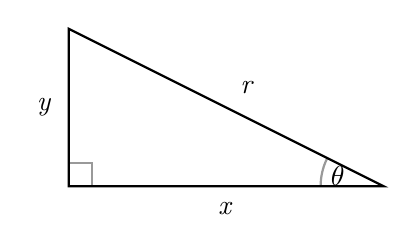
\begin{tikzpicture}[thick]
\coordinate (O) at (0,0);
\coordinate (A) at (4,0);
\coordinate (B) at (0,2);
\draw (O)--(B)--(A)--cycle;

\tkzLabelSegment[below=2pt](O,A){\textit{x}}
\tkzLabelSegment[left=2pt](O,B){\textit{y}}
\tkzLabelSegment[above right=2pt](A,B){\textit{r}}

\tkzMarkRightAngle[size=0.3,opacity=.4](A,O,B)% square angle here
\tkzLabelAngle[pos = 0.35](A,O,B){$$}

\tkzMarkAngle[size=0.8cm,%
opacity=.4](B,A,O)
\tkzLabelAngle[pos = 0.6](B,A,O){$\theta$}

% \tkzMarkAngle[size=0.7cm,%
% opacity=.4](O,B,A)
% \tkzLabelAngle[pos = 0.5](O,B,A){$\beta$}

\end{tikzpicture}
\end{center}
\tab
By the pythagorean theorem, it follows that $r^2=x^2+y^2$. Furthermore, by the definition of the sine and cosine functions, it follows that $\sin(\theta) = \frac{y}{r}$ and that $\cos(\theta) = \frac{x}{r}$. Dividing $r^2$ on both sides of the pythagorean theorem gives $\frac{x^2}{r^2} + \frac{y^2}{r^2} = 1$. Squaring both sides of the $\sin(\theta)$ and $\cos(\theta)$ definitions gives that $\sin^2(\theta) = \frac{y^2}{r^2}$ and that $\cos^2(\theta) = \frac{x^2}{r^2}$. Therefore, it follows from the pythagorean theorem, that $\sin^2(\theta) + \cos^2(\theta) = 1$.
\nextline
Next, consider $\sec^2(x)-\tan^2(x)$.
\begin{center}
\begin{tabular}{|l|l|}
\hline
\makecell{
	\Large{$\frac{1}{\cos^2(x)} - \frac{\sin^2(x)}{\cos^2(x)}$}
} & \makecell[l]{ Rewrite the tangent function as a quotient } \\
\hline
\makecell{
	\Large{$\frac{1-\sin^2(x)}{\cos^2(x)}$}
} & \makecell[l]{Combine the numerators of the quotients} \\
\hline
\makecell{
	\Large{$\frac{\cos^2(x)}{\cos^2(x)}$}
} & \makecell[l]{ Add the quotients and use the identity \\ $\sin^2(x)+\cos^2(x)=1\implies \cos^2(x)=1-\sin^2(x)$ } \\
\hline
\makecell{
	\large{$1$}
} & \makecell[l]{ Simplify the expression.} \\
\hline
\end{tabular}
\end{center}
\tab
Therefore, it follows that $\sec^2(x) - \tan^2(x) = 1$.
\nextline
A very similar argument can be made to show that $\csc^2(x)-\cot^2(x) = 1$ by manipulating the pythagorean identity as follows $\sin^2(x)+\cos^2(x)=1\implies\sin^2(x)=1-\cos^2(x)$.
\chapter{Integration Techniques}
\thm{Integration by Parts}{IntByPts}
\tab
Integration by parts is a method of undoing the product rule for derivatives. To start, let $u(x)$ and $v(x)$ be functions. Consider the following
\begin{equation*}
\ddx{u(x)\cdot v(x)} = u(x)\cdot\dfdx{v}{x} + v(x)\cdot\dfdx{u}{x}
\end{equation*}
\tab
To simplify this notation a little, assume that the $\d{x}$ part exists on the denominator to every corresponding $\d{u}$ and $\d{v}$ part. Then, this can be rewritten as
\begin{equation*}
\d{}\left[u\cdot v\right] = u\d{v} + v\d{u}
\end{equation*}
\tab
Integrating both sides and moving terms around yields the following.
\begin{flalign*}
& \int\d\left[u\cdot v\right] = \int u\d{v} + \int v\d{u} \\
& u\cdot v = \int u\d{v} + \int v\d{u} \\
& u\cdot v - \int v\d{u} = \int u\d{v}
\end{flalign*}
\tab
This is the traditional formula of integration by parts. When manipulating an integral, the functions $u$ and$\d{v}$ must be selected. As an example, consider the following integral.
\begin{equation*}
\int xe^x\d{x}
\end{equation*}
\tab
From this, take $u=x$ and$\d{v}=e^x\d{x}$. Then, the integral matches with the original setup.
\begin{equation*}
\int xe^x\d{x} = \int u\d{v}
\end{equation*}
\tab
To continue with the original formula, the integral of$\d{v}$ is required. As such, since $e^x$ is its own derivative, it is also its own integral. Thus, the conclusion that $v(x)=\d{v}\d{x}$ can be drawn. Furthermore, the derivative of $u$ is also required. This is rather simple, as the derivative of $x$ is 1 with respect to $x$. As such, we get that $\d{u}=1\cdot\d{x}$. Therefore, applying the integration by parts formula yields the following.
\begin{flalign*}
& \int u\d{v} = uv-\int v\d{u} \\
& \int xe^x = xe^x-\int e^x\d{x} \\
& = xe^x - e^x\\
& = e^x\left(x - 1\right) + C
\end{flalign*}
\tab
Powerful though this is, it is not uncommon that repeated integration by parts is required to solve a problem. As such, there exists a method that allows for a simple way to repeat the integration by parts technique as many times as required. 
\thm{D-I Method of Integration By Parts}{IntByPtsDI}
\tab
The idea of integration by parts is to break down an integral into separate parts for differentiation and integration. As such, a table can be constructed to hold the data for which parts are being integrated and which parts are being differentiated. In reality, it's an easier way to keep track of all integration by parts. As an example, consider the following integral.
\begin{equation*}
\int x^2\sin(x)\d{x}
\end{equation*}
\tab
To begin, setup a table consisting of columns for differentiation, integration, and multiples of $-1$. Note that since the original formula has a factor of $-1$, repeated application of integration by parts will stack them multiplicatively, and as such they alternate.
\nextline
Pick $x^2$ to differentiate and $\sin(x)$ to integrate.
\begin{center}
{\renewcommand{\arraystretch}{1.2}
\begin{tabular}{| c | c | c |}
\hline
   & D & I \\
\hline
+ & $x^2$ & $\sin(x)$ \\
\hline
- & $2x$ & $-\cos(x)$ \\
\hline
+ & $2$ & $-\sin(x)$ \\
\hline
- & $0$ & $\cos(x)$ \\
\hline
\end{tabular}
}
\end{center}
\tab
Firstly, to compute this, take the product of the diagonal from the left cell to the right cell (considering the top sign); this will be the $u\cdot v$ value from the integration by parts formula. Next, the product of a row itself is an integral. The third column (the one that reads ($+$, $2$, $-\sin(x)$)) is equivalent to $\int -2\sin(x)\d{x}$ and the second column (the one that reads ($-$, $2x$, $-\cos(x)$)) is equivalent to $\int 2x\cos(x)\d{x}$ since the negatives will cancel out.
\nextline
There are a couple of very important things to note. If a $0$ appears in the differentiation column, then the process should stop. This is because, the product of that integral is 0, and the product of the diagonal will also be 0.
\nextline
Thus, to finish solving the integral, since a $0$ appears in the differentiation column, take the product of the diagonal of every row as follows.
\begin{center}
\begin{tabular}{c  c  c}

   & D & I \\ \\
+ & $x^2$\tikzmark{aa} & $\sin(x)$ \\
& & \tikzmark{ba} \\
- & $2x$\tikzmark{ab} & $-\cos(x)$ \\
& & \tikzmark{bb}\\
+ & $2$\tikzmark{ac} & $-\sin(x)$ \\
& & \tikzmark{bc}\\
- & $0$ & $\cos(x)$\\
\end{tabular}
  \begin{tikzpicture}[overlay, remember picture, yshift=.25\baselineskip, shorten >=.5pt, shorten <=.5pt]
    \draw [->] ([yshift=.75pt]{pic cs:aa}) -- ({pic cs:ba});
    \draw [->] ([yshift=.75pt]{pic cs:ab}) -- ({pic cs:bb});
	\draw [->] ([yshift=.75pt]{pic cs:ac}) -- ({pic cs:bc});
  \end{tikzpicture}
\end{center}
\tab
From this, as mentioned above, multiplying the rows (with consideration of the sign from which the arrow comes from) will provide the solution.
\begin{flalign*}
& \int x^2\sin(x)\d{x} = -x^2\cos(x) -2x\cdot(-\sin(x)) + 2\cos(x) \\
& = -x^2\cos(x) + 2x\sin(x) + 2\cos(x) \\
& = \cos(x)(2-x^2) + 2x\sin(x) + C 
\end{flalign*}
\tab
This is nothing but storing the repetitive usage of integration by parts in a table. It is also refered to as The Tabular Method for Repeated Integration By Parts.
\thm{U-Substitution}{USUB}
\tab
Consider the chain rule of derivatives:
\begin{equation*}
\ddx{f(g(x))} = f^\prime(g(x))g^\prime(x)
\end{equation*}
\tab
If one were to attempt to reverse this, the situation would require an integral of the following type:
\begin{equation*}
f(g(x)) + C = \int f^\prime(g(x))g^\prime(x) \d{x}
\end{equation*}
\tab
As such, given a function $A(x)$, the integral may be easier to evaluate when reversing the chain rule. That is to say, given some choice of $B(x)$, the following is true.
\begin{equation*}
\int A(x)\d{x} = \int A(B(x))B^\prime(x)\d{x}
\end{equation*}
\subsection*{Example 1}
\tab
Consider the following:
\begin{equation*}
\int \cos\left(x^2\right)\cdot2x\d{x}
\end{equation*}
\tab
Consider the function $f(x)=x^2$. Notice that $f^\prime(x) = 2x$, and thus, this integral matches one of the form
\begin{equation*}
\int A(B(x))\cdot B^\prime(x)\d{x}
\end{equation*}
\tab
From this, let $A(x)=\cos(x)$ and $B(x)=x^2$. Then, note that since $\ddx{\sin(x)}=\cos(x)$, that the integral will evaluate to the follwing:
\begin{equation*}
\int \cos\left(x^2\right)\cdot2x\d{x} = \sin\left(x^2\right) + C
\end{equation*}
\tab
The more traditional way of writing this is to say ``Let $u=x^2$''. Differentiating $u$ yields $\d{u}=2x\d{x}$, and thus the $2x\d{x}$ term in the integral can be replaced with $\d{u}$. Therefore, the integral can be rewritten as
\begin{equation*}
\int\cos\left(x^2\right)\cdot 2x\d{x} = \int\cos(u)\d{u}
\end{equation*}
\tab
Evaluating the integral gives $\sin(u) + C$. Since $u=x^2$, reversing the substitution yields $\sin\left(x^2\right)+C$, resulting in the same answer.
\subsection*{Example 2}
\tab
Consider the following
\begin{equation*}
\int \ln(x)^5\d{x}
\end{equation*}
\tab
In this case, note that $\frac{1}{x}$ --- the derivative of $\ln(x)$ --- is nowhere present within the integral. However, this does not mean that a substitution can't be made.
\begin{flalign*}
& \text{Let } u=\ln(x) \iff e^u = x \\
& \d{u} = \frac{1}{x}\d{x} \\
& x\d{u} = \d{x} \\
& e^u\d{u} = \d{x}
\end{flalign*}
\tab
Thus, a similar substitution can be made as before, where now $\d{x}=e^u\d{u}$. This results in the following integral
\begin{flalign*}
\int \ln(x)^2\d{x} = \int u^5e^u\d{u}
\end{flalign*}
\tab
From here, the \hyperref[sec:IntByPtsDI]{D-I Method} for \hyperref[sec:IntByPts]{Integration by Parts}. Since $e^x$ is its own integral, that can be chosen for integration.
\begin{center}
{\renewcommand{\arraystretch}{1.2}
\begin{tabular}{|c|c|c|}
\hline
& D & I \\
\hline
+ & $u^5$ & $e^u$ \\
\hline
- & $5u^4$ & $e^u$ \\
\hline
+ & $20u^3$ & $e^u$ \\
\hline
-  & $60u^2$ & $e^u$ \\
\hline
+ & $120u$ & $e^u$ \\
\hline
- & $120$ & $e^u$ \\
\hline
+ & $0$ & $e^u$ \\
\hline
\end{tabular}
}
\end{center}
\tab
Since there's a 0 in the differentiation column, the result of the integral can is the sum of the products of the diagonals. As such, it follows that
\begin{flalign*}
& \int u^5e^u \d{u} = u^5e^u - 5u^4e^u + 20u^3e^u -60u^2e^u+120ue^u - 120e^u\\
& = e^u\left(u^5 - 5u^4 + 20u^3 - 60u^2 + 120u - 120\right)
\end{flalign*}
\tab
Undoing the substitution yields the following result
\begin{flalign*}
& \int \ln(x)^5\d{x} \\
& = e^{\ln(x)}\left(\ln(x)^5 - 5\ln(x)^4 + 20\ln(x)^3 - 60\ln(x)^2 + 120\ln(x) - 120\right) \\
& = x\left(\ln(x)^5 - 5\ln(x)^4 + 20\ln(x)^3 - 60\ln(x)^2 + 120\ln(x) - 120\right) + C
\end{flalign*}
\thm{Trigonometric Substitutions}{TrigSub}
\tab
Often times while performing integration, certain substitutions can be made that might not seem obvious at first, but greatly reduce the difficulty of the problem. In general, this is the art of integration: finding that one substitution that reduces greatly the difficulty. When dealing with quadratics, there are trigonometric substitutions that one might not initially consider, but can reduce difficulty using certain identities. Unlike other sections of this document, there will be no formal proofs. Instead, this section will consist of guidelines for substitutions.
\begin{center}
\begin{tabular}{|l|l|l|l|}
\hline
Expression & Substitution & Identity & Explanation \\
\hline
$\sqrt{x^2+a^2}$ & $x=a\tan(\theta)$ & $\sec^2(\theta)-\tan^2(\theta)=1$ &
\makecell[l]{
	Performing this substitution allows for \\
	factoring out the $a$ and using the \\
	identity to get a $a\sec^2(\theta)$ to cancel out \\
	the square root.
} \\
\hline
$\sqrt{x^2-a^2}$ & $x=a\sec(\theta)$ & $\sec^2(\theta)-\tan^2(\theta)=1$ &
\makecell[l]{
	Performing this substitution allow for \\
	factoring out the $a$ and using the \\
	identity to get $a\tan^2(\theta)$ to cancel out \\
	the square root.
} \\
\hline
$\sqrt{a^2-x^2}$ & $x=a\sin(\theta)$ & $\sin^2(x)+\cos^2(x) = 1$ &
\makecell[l]{
	Performing this substitution allow for \\
	factoring out the $a$ and using the identity \\
	to get $a\cos^2(\theta)$ to cancel out \\
	the square root.
} \\
\hline
\end{tabular}
\end{center}
\tab
It is also important to note that whichever function is chosen for the substitution, that the complementary function will also work. As an example, if one chooses to use $x=a\sec(\theta)$ as the substitution, that $x=a\csc(\theta)$ will work since the identity holds for the complementary set as well.
\chapter{The Integral}
\tab
This document will focus on finding the derivative of the function $\sqrt{ax^2+bx+c}$. That is to say, this document focuses on the evaluation of
$$\int \sqrt{ax^2+bx+c} \d{x}$$
\tab
All tools that are used to solve this problem have been previously discussed in the previous chapters and will be fully accessible by links.
\nextline
To start, consider the quadratic function $ax^2+bx+c$. The \hyperref[sec:CTS]{Completing The Square} technique allows for the rewriting of the quadratic into a vertex form. This can be done as follows:
\begin{center}
{\renewcommand{\arraystretch}{1.2}
\begin{tabular}{| l | l |}
\hline
\makecell{
	\large{$a\left(x^2+\frac{b}{a}x\right) + c$}
}
& \makecell[l]{Start by factoring out the coefficient of the $x^2$ term. \\ Factoring it out of the $c$ term is not required, \\ as it does not affect the completing the square process.} \\ 
\hline
\makecell{
	\Large{$\frac{b}{a} = 2y$}
}
& \makecell[l]{Match the $x$ coefficient to that \\ from the form $x^2+2xy+y^2$.} \\
\hline
\makecell{
	\Large{$\frac{b}{2a} = y$}
}
& \makecell[l]{Isolate for the $y$ term} \\ 
\hline
\makecell{
	\Large{$\frac{b^2}{4a^2} = y^2$}
}
& \makecell[l]{Square both sides to find the corresponding $y^2$ value} \\ 
\hline
\makecell{
	\large{$a\left(x^2+\frac{b}{a}x+\frac{b^2}{4a^2}-\frac{b^2}{4a^2}\right)+c$}
}
& \makecell[l]{Add and subtract the corresponding $y^2$ value.} \\
\hline
\makecell{
	\large{$a\left(x^2+\frac{b}{a}x+\frac{b^2}{4a^2}\right) + c - \frac{b^2}{4a}$}
}
& \makecell[l]{Move the last term out of the factoring \\ by multiplying it by $a$.} \\
\hline
\makecell{
	\large{$a\left(x+\frac{b}{2a}\right)^2 + c - \frac{b^2}{4a}$}
}
& \makecell[l]{Factor everything within the parentheses.} \\
\hline
\end{tabular}
}
\end{center}
\tab
From this, the original integral is now equivalent to the following.
\begin{equation*}
\int\sqrt{a\left(x+\frac{b}{2a}\right)^2 + c - \frac{b^2}{4a}}\d{x}
\end{equation*}
\tab
Combining the fraction in the square root with the $c$ term results in
\begin{equation*}
\bigintss\sqrt{a\left(x+\frac{b}{2a}\right)^2 + \frac{4ac-b^2}{4a}}\d{x}
\end{equation*}
\tab
From here, factor out a $\frac{1}{4a}$ term from everything in the square root.
\begin{equation*}
\bigintss\sqrt{\frac{1}{4a}\left(4a^2\left(x+\frac{b}{2a}\right)^2+4ac-b^2\right)}\d{x}
\end{equation*}
\tab
Now, the $\frac{1}{4a}$ term can be taken out of the square root, resulting in $\frac{1}{2\sqrt{a}}$, and subsequently removed from the integral. Furthermore, the fraction $x+\frac{b}{2a}$ can be combined, resulting in $\frac{2ax+b}{2a}$. This yields the following result.
\begin{equation*}
\frac{1}{2\sqrt{a}}\bigintss\sqrt{4a^2\left(\frac{2ax+b}{2a}\right)^2 + 4ac-b^2}\d{x}
\end{equation*}
\tab
The factor of $4a^2$ can be moved into the adjacent term, resulting in $\frac{(2a)(2ax+b)}{2a}$. This results in the following.
\begin{equation*}
\frac{1}{2\sqrt{a}}\bigintss\sqrt{(2ax+b)^2 + 4ac-b^2}\d{x}
\end{equation*}
\tab
To continue, one can introduce a \hyperref[sec:USUB]{U-Substitution} as follows. Furthermore, we can introduce a new variable to represent the remaining constant. Since this variable is just a constant with respect to the integral, no change needs to be made.
\begin{flalign*}
& \text{Let } u=2ax+b \iff x=\frac{u-b}{2a} \\
& \d{u} = 2a\d{x} \\
& \frac{\text{d}u}{2a} = \d{x} \\
& q = \sqrt{4ac-b^2} \\
\end{flalign*}
\tab
Since $\frac{1}{2a}$ is a constant, it can be removed from the inside of the integral. Using this substitution, the integral becomes the following.
\begin{equation*}
\frac{1}{4a\sqrt{a}}\int\sqrt{u^2+q^2}\d{u}
\end{equation*}
\tab
A \hyperref[sec:TrigSub]{Trigonometric Substitution} can be used to proceed from here.
Take $u=q\tan(\theta)$ and proceed with a u-substitution.
\begin{flalign*}
& u=q\tan(\theta) \\
& \d{u} = q\sec^2(\theta)\d{\theta} \\
& \frac{q}{4a\sqrt{a}}\int\sqrt{q^2\tan^2(\theta) + q^2}\sec^2(\theta)\d{\theta} \\
\end{flalign*}
\tab
From this, factoring out the $q$ will allow for the use of \hyperref[sec:TrigIden]{Trigonometric Identities}.
\begin{center}
\begin{tabular}{| l | l |}
\hline
\makecell{
	$\frac{q}{4a\sqrt{a}}\bigintss\sqrt{q^2\left(\tan^2(\theta) + 1\right)}\sec^2(\theta)\d{\theta}$
}
&
\makecell[l]{
	Factor out $q$ from inside the big root.
} \\
\hline
\makecell{
	$\frac{q}{4a\sqrt{a}}\bigintsss\sqrt{q^2\sec^2(\theta)}\sec^2(\theta)\d{\theta}$
}
&
\makecell[l]{
	Use the identity $\tan^2(\theta) = \sec^2(\theta)-1$.
} \\
\hline
\makecell{
	$\frac{q}{4a\sqrt{a}}\bigintsss q\sqrt{\sec^2(\theta)}\sec^2(\theta)\d{\theta}$
}
&
\makecell[l]{
	Factor out the $q^2$ from the square root as $q$.
} \\
\hline
\makecell{
	$\frac{q^2}{4a\sqrt{a}}\bigintsss\sec(\theta)\sec^2(\theta)\d{\theta}$
} &
\makecell[l]{
	Factor out the constant term from the integral.
} \\
\hline
\makecell{
	\Large{$\frac{q^2}{4a\sqrt{a}}\mathcal{I}$}
} &
\makecell[l]{
	Let $\mathcal{I}=\bigintsss\sec^3(\theta)\d{\theta}$. \\ This will be useful later on.
} \\
\hline
\end{tabular}
\end{center}
\tab
From this, it is easy to perform \hyperref[sec:IntByPts]{Integration by Parts}. To do this, differentiate $\sec(\theta)$ and integrate $\sec^2(\theta)$. Integrating $\sec^2(\theta)$ can be easily done using a \hyperref[sec:USUB]{U-Substitution}.
\begin{center}
\begin{tabular}{|l|l|}
\hline
\makecell{
	Let $m=\tan(\theta)$ \\
	$\d{m} = \sec^2(\theta)\d{\theta}$
} & \makecell[l]{Apply a substitution using $m$ \\ since $u$ was already used.} \\
\hline
\makecell{
	$\int\sec^2(\theta)\d{\theta} = \int \text{d}m$ 
} &
\makecell[l]{
	The entire integral is equal to $\d{m}$.
} \\
\hline
\makecell{
	$\int \text{d}m = m = \tan(\theta) + C$
} &
\makecell[l] {
	Integrate and undo the substitution.
} \\
\hline
\end{tabular}
\end{center}
\tab
From here, we can continue with integration by parts. To reduce confusion, when using the integration by parts formula, the position of $u$ will be replaced with $g$, since $u$ was already used in a previous substitution. Choose $g=\sec(\theta)$ and $\text{d}v = \sec^2(\theta)$. By the work shown above, $v=\tan(\theta)$. Differentiating $\sec(\theta)$ gives that $\text{d}g = \tan(\theta)\sec(\theta)$. Thus, by the integration by parts formula, the integral becomes the following.
\begin{equation*}
\frac{q^2}{4a\sqrt{a}}\int\sec(\theta)\sec^2(\theta)\d{\theta} = \frac{q^2}{4a\sqrt{a}}\left(\sec(\theta)\tan(\theta) - \int \tan^2(\theta)\sec(\theta)\d{\theta}\right)
\end{equation*}
\tab
$\tan^2(\theta)$ can be written as $\sec^2(\theta)-1$, and as such, the right-hand integral becomes the following.
\begin{equation*}
\frac{q^2}{4a\sqrt{a}}\int\sec(\theta)\sec^2(\theta)\d{\theta} = \frac{q^2}{4a\sqrt{a}}\left(\sec(\theta)\tan(\theta) - \int \sec(\theta)\left(\sec^2(\theta)-1\right)\d{\theta}\right)
\end{equation*}
\tab
Notice how after distributing the $\sec(\theta)$ into $\sec^2(\theta)-1$, that another $\sec^3(\theta)$ integral appears. Since $\int\sec^3(\theta)\d{\theta}=\mathcal{I}$, it can be manipulated algebraically as follows.
\begin{flalign*}
& \frac{q^2}{4a\sqrt{a}}\mathcal{I} = \frac{q^2}{4a\sqrt{a}}\left(\sec(\theta)\tan(\theta) - \mathcal{I} + \int\sec(\theta)\d{\theta}\right) \\
& 2\frac{q^2}{4a\sqrt{a}}\mathcal{I} = \frac{q^2}{4a\sqrt{a}}\sec(\theta)\tan(\theta) + \frac{q^2}{4a\sqrt{a}}\int\sec(\theta)\d{\theta}
\end{flalign*}
\tab
To continue, a value needs to be found for $\int\sec(\theta)\d{\theta}$.
\begin{center}
\begin{tabular}{| l | l |}
\hline
\makecell{
	\large{$\bigintss\sec(\theta)\cdot\frac{\tan(\theta)+\sec(\theta)}{\tan(\theta)+\sec(\theta)}\d{\theta}$}
} &
\makecell[l]{
	To begin, multiply and divide the \\
	integrand by $\tan(\theta)+\sec(\theta)$.
} \\
\hline
\makecell{
	\large{$\frac{\sec(\theta)\tan(\theta)+\sec^2(\theta)}{\tan(\theta)+\sec(\theta)}\d{\theta}$}
} & 
\makecell[l]{
	Expand the numerator of the quotient.
} \\
\hline
\makecell{
	Let $r=\tan(\theta)+\sec(\theta)$ \\
	$\text{d}r = \sec(\theta)\tan(\theta)+\sec^2(\theta)\text{d}\theta$ \\
	\large{$\int\frac{1}{r}\d{r}$}
} &
\makecell[l]{
	Perform a u-substitution to simplify \\
	the denominator and cancel the numerator.
} \\
\hline
\makecell{
	\large{$\ln\abs{r}$}
} &
\makecell[l]{
	Integrate $\frac{1}{r}$ to get the natural log. \\
	Note that since $\ln(x)$ only exists for $x>0$, \\
	but $\frac{1}{x}$ exists everywhere except 0. \\
	Thus, the result will be contained in absolute values.
} \\
\hline
\makecell{
	\large{$\ln\abs{\tan(\theta)+\sec(\theta)}+C$}
} &
\makecell[l]{
	Undo the substitution, finalizing the integral.
} \\
\hline
\end{tabular}
\end{center}
\tab
With the integral of $\sec(\theta)$ acquired, the final result can now be put together.
\nextline
To start, divide by $2$ to acquire the original integral
\begin{equation*}
\frac{q^2}{4a\sqrt{a}}\mathcal{I} = \frac{1}{2}\left(\frac{q^2}{4a\sqrt{a}}\sec(\theta)\tan(\theta) + \frac{q^2}{4a\sqrt{a}}\int\sec(\theta)\d{\theta}\right)
\end{equation*}
\tab
The integral of $\sec(\theta)$ can be substituted in, resulting in the following.
\begin{equation*}
\frac{q^2}{4a\sqrt{a}}\mathcal{I} = \frac{q^2}{8a\sqrt{a}}\left(\sec(\theta)\tan(\theta) + \ln\abs{\tan(\theta)+\sec(\theta)}\right)
\end{equation*}
\tab
The substitution $u=q\tan(\theta)$ can now be undone. Firstly, note that $\frac{u}{q}=\tan(\theta)$. Next, a trigonometric identity can be used to find the corresponding formula $\sqrt{1+\frac{u^2}{q^2}} = \sec(\theta)$.
\begin{equation*}
\frac{q^2}{4a\sqrt{a}}\mathcal{I} = \frac{q^2}{8a\sqrt{a}}\left(\sqrt{1+\frac{u^2}{q^2}}\cdot\frac{u}{q} + \ln\abs{\frac{u}{q}+\sqrt{1+\frac{u^2}{q^2}}}\right)
\end{equation*}
\tab
From here, the substitution $u=2ax+b$ can be undone to acquire the following. 
\begin{equation*}
\frac{q^2}{4a\sqrt{a}}\mathcal{I} = \frac{q^2}{8a\sqrt{a}}\left(\sqrt{1+\frac{\left(2ax+b\right)^2}{q^2}}\cdot\frac{2ax+b}{q} + \ln\abs{\frac{\left(2ax+b\right)}{q}+\sqrt{1+\frac{\left(2ax+b\right)^2}{q^2}}}\right)
\end{equation*}
\tab
Finally, the substitution $q=\sqrt{4ac-b^2}$ can be undone. Therefore, the final result is as follows.
\begin{equation*}
\frac{4ac-b^2}{8a\sqrt{a}}\left(\sqrt{1+\frac{(2ax+b)^2}{4ac-b^2}}\cdot\frac{2ax+b}{\sqrt{4ac-b^2}} + \ln\abs{\sqrt{1+\frac{(2ax+b)^2}{4ac-b^2}}+\frac{2ax+b}{\sqrt{4ac-b^2}}}\right) + C
\end{equation*}
\end{document}